% Requires \usepackage{placeins} in main.tex.

\section{Evaluation}
\label{sec:evaluation}

\subsection{Questions, evidence layers, and metrics}
\label{sec:setup}

We ask four questions.
\begin{description}
\setlength{\itemsep}{0pt}
\setlength{\parskip}{0pt}

\item[RQ1]
How does operand-constrained auditing compare with ordinary
numeric, trace-rule, anomaly, and model-based checks?

\item[RQ2]
Does the frozen audit transfer across datasets, and how does
closure depth expose its derivation--collision trade-off?

\item[RQ3]
Which semantic changes remain invisible to execution-result
equality, and which complementary checks detect them?

\item[RQ4]
Do replay certificates improve the quality of completed episodes
delivered to users or downstream systems?
\end{description}

\etitle{Evidence layers.}
ConvFinQA and MultiHiertt evaluate the bounded-closure component
using program-labelled numerical derivations and aligned
cross-example answer substitutions. WikiSQL evaluates the
task-specific semantic interface through controlled program
perturbations. KramaBench and DABstep evaluate completed
data-agent episodes through restricted replay, failure
localization, and selective delivery. The KramaBench human label
is a composite deliverability judgement: it asks whether the
stated answer follows from the cited data through the recorded
computation and addresses the requested quantity.

\begin{table}[t]
\centering
\caption{Evaluation layers and their primary roles. Size reports
total/evaluable instances where the distinction applies.}
\label{tab:datasets}
\scriptsize
\renewcommand{\arraystretch}{1.05}
\setlength{\tabcolsep}{2.5pt}
\begin{tabularx}{\columnwidth}{@{}l l r X@{}}
\toprule
Layer & Dataset & Size & Primary use \\
\midrule
Closure
& ConvFinQA
& 388/386
& Arithmetic audit and baselines \\

Closure
& MultiHiertt
& 7,830/6,301
& Transfer and depth stress \\

Semantic
& WikiSQL
& 500/2,715
& Same-output program changes \\

Live audit
& KramaBench
& 166
& Replay and selective delivery \\

Live audit
& DABstep
& 60
& Completed-episode transfer \\

Human
& KramaBench
& 40/39
& Deliverability and escalation \\
\bottomrule
\end{tabularx}
\end{table}

\etitle{Metrics.}
For program-labelled examples, \emph{reference-derivation recall}
is the fraction of supported derivations that receive a closure
certificate, and \emph{cross-example rejection} is the fraction
of aligned unsupported substitutions that do not receive one.
For WikiSQL, \emph{perturbation detection} is the fraction of
modified queries identified as changed, while the false-positive
rate is measured on unmodified reference queries. For selective
delivery, \emph{coverage} is the fraction of evaluable episodes
delivered; \emph{delivered support} is the fraction of delivered
episodes judged supported by human annotators;
\emph{supported-case retention} is the fraction of all
human-supported episodes retained; and \emph{mean delivered
score} averages the benchmark's official score over delivered
episodes.

\etitle{Baselines.}
Numeric baselines include exact operand matching, one-operation
derivability, and closure over all numbers in the cited context.
Trace rules check execution success, citation resolution,
declared-read coverage, and unrestricted replay. Anomaly baselines
use robust MAD distance, Isolation Forest
\citep{liu2008isolation}, Local Outlier Factor
\citep{breunig2000lof}, and one-class SVM
\citep{scholkopf2001support}. Their thresholds use only the
60-example calibration seed and retain at least 90\% supported
derivations on that seed. A supervised logistic model provides an
upper baseline. No anomaly feature contains the audit verdict or
benchmark answer.

\etitle{Evidence-aware judge.}
A local Qwen3.6-35B judge receives the question, declared evidence
metadata, observed reads, program summary, execution status,
recomputed output, and stated answer. It receives neither benchmark
gold nor \ledger labels. Three temperature-zero repeats measure
response stability. Transferred human records omit most raw rows
and complete program bodies, so that subset remains a
limited-evidence diagnostic.

\subsection{RQ1: Program-reached operands separate derivations
from numeric coincidence}
\label{sec:rq1}

\begin{figure*}[!t]
\centering
\begin{minipage}[t]{0.316\textwidth}
\centering
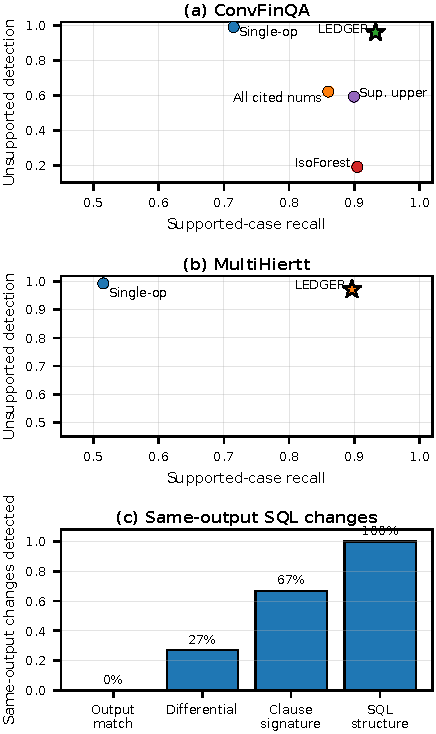
\includegraphics[
  width=\linewidth,
  trim=0 234.8bp 0 0,
  clip
]{fig_baselines_semantics_3panel.pdf}
\end{minipage}
\hfill
\begin{minipage}[t]{0.316\textwidth}
\centering
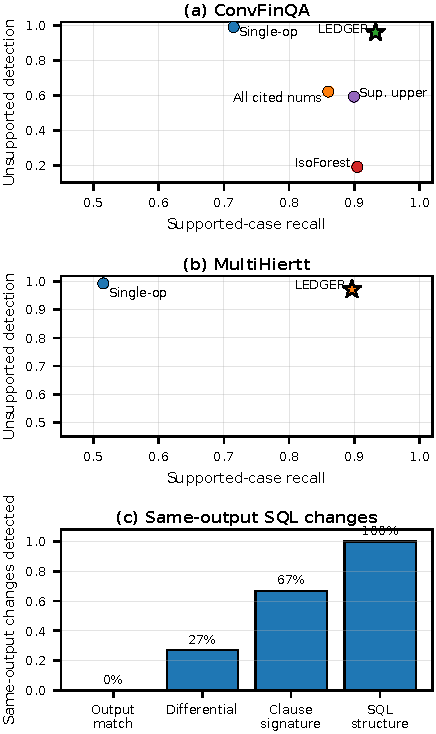
\includegraphics[
  width=\linewidth,
  trim=0 117.4bp 0 117.4bp,
  clip
]{fig_baselines_semantics_3panel.pdf}
\end{minipage}
\hfill
\begin{minipage}[t]{0.316\textwidth}
\centering
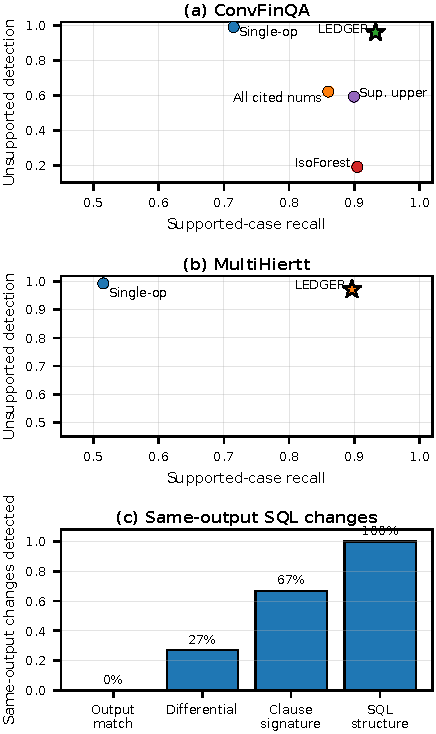
\includegraphics[
  width=\linewidth,
  trim=0 0 0 234.8bp,
  clip
]{fig_baselines_semantics_3panel.pdf}
\end{minipage}
\caption{%
Operand-constrained auditing on ConvFinQA and MultiHiertt,
together with the semantic complement on WikiSQL.
Panels (a,b) report reference-derivation recall and
cross-example rejection; panel (c) reports detection on
same-output SQL changes.}
\label{fig:baselines}
\end{figure*}

\etitle{Trace-local closure preserves derivations and suppresses
unrelated numbers.}
ConvFinQA supplies 386 evaluable reference derivations and aligned
cross-example substitutions; MultiHiertt supplies 6,301 aligned
pairs. The frozen checker uses program-reached operands, five
operations, depth 2, and relative tolerance $10^{-4}$. It recovers
93.3\% and 89.6\% of the reference derivations on ConvFinQA and
MultiHiertt, while rejecting 96.1\% and 97.2\% of the corresponding
cross-example substitutions. Closure over all cited-context
numbers recovers additional derivations over one-operation
checking, but also admits many unrelated numeric coincidences.

\begin{table}[t]
\centering
\caption{ConvFinQA baselines on the held-out remainder.}
\label{tab:baselines}
\scriptsize
\setlength{\tabcolsep}{3pt}
\begin{tabular}{@{}lcc@{}}
\toprule
Method
& Derivation recall
& Cross-example rejection \\
\midrule
Single operation
& 276/386 (0.715)
& 383/386 (0.992) \\

All cited numbers
& 332/386 (0.860)
& 240/386 (0.622) \\

Isolation Forest
& 351/388 (0.905)
& 74/388 (0.191) \\

Supervised upper
& 349/388 (0.899)
& 230/388 (0.593) \\

\textbf{\ledger}
& \textbf{360/386 (0.933)}
& \textbf{371/386 (0.961)} \\
\bottomrule
\end{tabular}
\end{table}

\etitle{Standard anomaly scores do not produce a derivation
witness.}
Isolation Forest, Local Outlier Factor, and one-class SVM retain
most supported examples but reject only 13.7--19.8\% of the
cross-example substitutions. Their trace features identify unusual
executions, but do not establish that the answer follows from the
program-reached values. Restricting closure to those operands
preserves the relevant search space and removes unrelated context
numbers before recursive expansion.

\subsection{RQ2: Closure depth recovers derivations and expands
the collision surface}
\label{sec:rq2}

\begin{figure}[!t]
\centering
\begin{minipage}[t]{0.49\columnwidth}
\centering
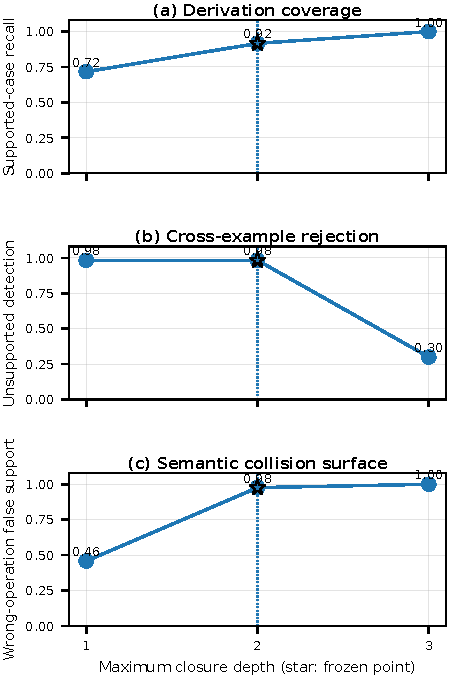
\includegraphics[
  width=\linewidth,
  trim=0 216.8bp 0 0,
  clip
]{fig_depth_ablation_3panel.pdf}
\end{minipage}
\hfill
\begin{minipage}[t]{0.49\columnwidth}
\centering
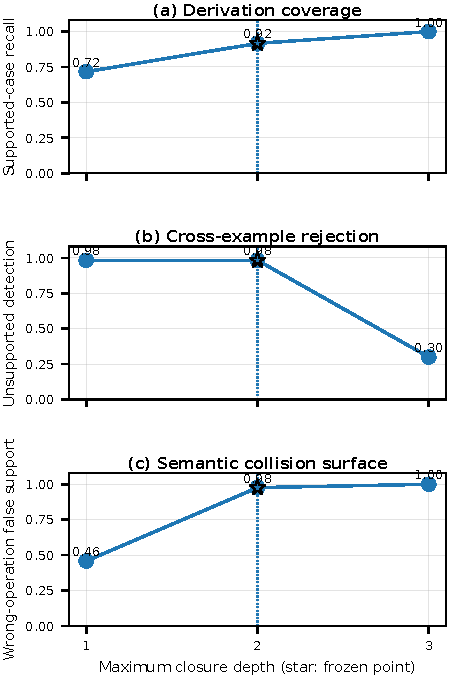
\includegraphics[
  width=\linewidth,
  trim=0 108.4bp 0 108.4bp,
  clip
]{fig_depth_ablation_3panel.pdf}
\end{minipage}

\vspace{1pt}

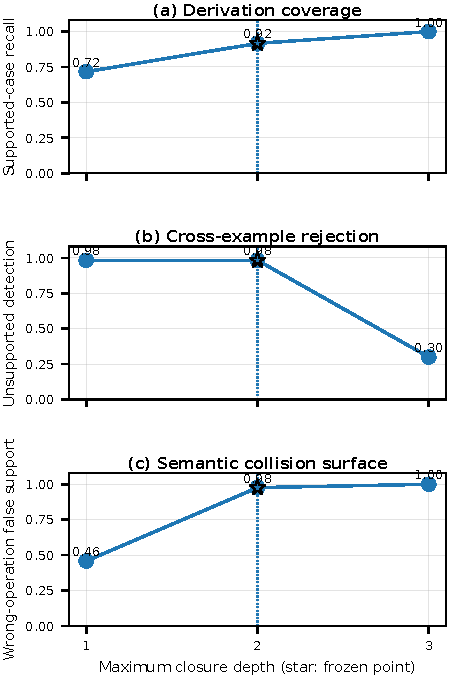
\includegraphics[
  width=0.72\columnwidth,
  trim=0 0 0 216.8bp,
  clip
]{fig_depth_ablation_3panel.pdf}
\caption{%
Effect of closure depth on derivation coverage,
cross-example rejection, and wrong-operation false support.
The star marks the frozen depth-2 setting.}
\label{fig:ablation}
\end{figure}

\etitle{Depth 2 captures short programs while retaining
cross-example rejection.}
We stratify MultiHiertt by reference-program depth and vary closure
depth on the disjoint ConvFinQA calibration seed. Most remaining
MultiHiertt misses correspond to programs deeper than the frozen
bound: 72.3\% of misses exceed depth 2. Increasing calibration
depth from 1 to 3 recovers every supported seed derivation, while
cross-example rejection falls sharply
(Figure~\ref{fig:ablation}a,b).

\etitle{Additional depth enlarges the semantic collision surface.}
We replace each ConvFinQA answer with the result of a different
operation over the same operands. Across all 382 substitutions,
only 9 are rejected; none of the 347 substitutions within the
frozen operation vocabulary and depth is rejected. Deeper closure
accepts still more variants because the altered answers remain
derivable from the same values
(Figure~\ref{fig:ablation}c). Closure therefore records arithmetic
derivability, while operation identity remains a semantic property.

\subsection{RQ3: Structural validation detects same-output
program changes}
\label{sec:rq3}

\etitle{Execution-result equality misses semantic changes.}
From 500 executable WikiSQL development examples, we construct
2,715 perturbations that alter aggregation, projection, predicate
column or value, or predicate presence. Execution-result equality
misses 466 perturbations because the modified and reference
programs return the same result on the original database.

\etitle{Program structure complements replay.}
Normalized SQL structure detects all 2,715 perturbations with no
false positives on the 500 unmodified reference queries. On a
100-case same-output sample, operator/clause signatures detect
67 changes and differential execution detects 27, while
original-database output comparison detects none
(Figure~\ref{fig:baselines}c). Structural comparison observes the
changed program directly; execution on database variants succeeds
when the variants separate the candidate and reference programs.
SQL deployments can therefore instantiate $V_q$ through structural
and test-suite methods \citep{zhong2020testsuite}; model-based
metrics such as FLEX remain an alternative when reference programs
are unavailable \citep{kim2025flex}.

\subsection{RQ4: Replay certificates support selective delivery}
\label{sec:rq4}

\begin{figure}[!t]
\centering
\begin{minipage}[t]{0.49\columnwidth}
\centering
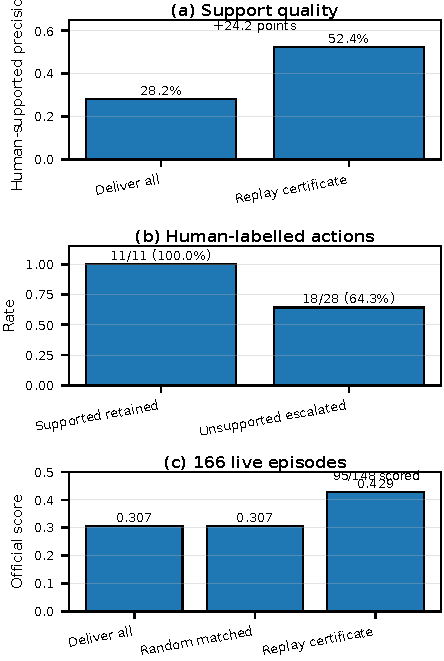
\includegraphics[
  width=\linewidth,
  trim=0 211.5bp 0 0,
  clip
]{fig_governance_3panel.pdf}
\end{minipage}
\hfill
\begin{minipage}[t]{0.49\columnwidth}
\centering
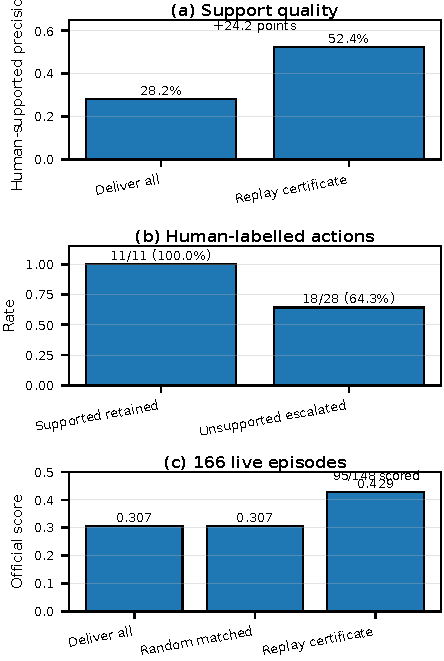
\includegraphics[
  width=\linewidth,
  trim=0 105.7bp 0 105.7bp,
  clip
]{fig_governance_3panel.pdf}
\end{minipage}

\vspace{1pt}

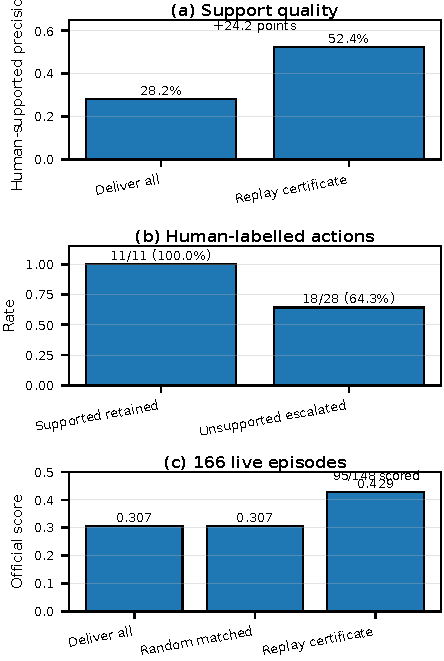
\includegraphics[
  width=0.72\columnwidth,
  trim=0 0 0 211.5bp,
  clip
]{fig_governance_3panel.pdf}
\caption{%
Replay-based selection improves delivered support, retains
human-supported episodes, escalates unsupported episodes, and
raises mean delivered score at partial coverage.}
\label{fig:governance}
\end{figure}

\etitle{Replay status provides a human-facing delivery signal.}
The live corpus contains 166 KramaBench and 60 DABstep episodes.
Among 39 KramaBench episodes with clear human labels, delivering
only replay-certified episodes retains all 11 supported cases and
escalates 18 of 28 unsupported cases. The proportion of delivered
answers judged supported consequently rises from 28.2\% to 52.4\%
(Figure~\ref{fig:governance}a,b). The remaining replay-certified
but human-unsupported episodes reproduce a value through programs
that address the wrong quantity, scope, or operation, consistent
with the separation between provenance and semantics.

\etitle{The same certificate improves score at partial coverage.}
Among 148 KramaBench episodes with finite official scores,
replay-certificate delivery selects 95 episodes, corresponding to
64.2\% coverage. Their mean official score is 0.429, compared with
0.307 for delivering all episodes and 0.307 for uniformly random
selection at the same size
(Figure~\ref{fig:governance}c). The policy changes which completed
episodes are delivered; it does not modify host-agent source
selection, program generation, or execution.

\subsection{Runtime, determinism, and model baseline}
\label{sec:runtime}

\etitle{Deterministic bookkeeping is small relative to host
execution.}
Across 500 saved records, the audit adds sub-millisecond median
bookkeeping and makes zero model calls. Five independent repeats
over 100 records produce identical execution-provenance outcomes.
These measurements cover record parsing, comparison, and closure
over saved traces; they exclude host-agent execution and external
data loading.

\etitle{The model judge remains a diagnostic baseline.}
An evidence-aware 35B judge shows label disagreement,
structured-output failures, and occasional repeat flips. The
complete counts appear in Appendix~\ref{app:tables}. Judge outputs
do not alter the deterministic execution-provenance status.

% \FloatBarrier